\chapter{Contagens de categorias de um ficheiro \hologo{BibTeX}}
\label{chap:a}

\section{Análise do Problema}
Neste primeiro problema, pretende-se analisar um documento \hologo{BibTeX} e fazer as
contagens das respetivas categorias, tais como artigos, teses de mestrado,
manuais, etc. O resultado tem que constar num ficheiro \texttt{HTML}.


\label{sec:ap:a}

\subsection{Especificação dos requisitos}
\label{sec:spec:a}
Existem pelo menos 14 tipos de entradas bibliográficas no \hologo{BibTeX},
podendo haver algumas extensões ou pacotes que possuam outras --- como por exemplo
o \textsc{Bib}\LaTeX{}.
Note-se que, a distinção entre o formato de ficheiro \hologo{BibTeX}
e o programa \hologo{BibTeX} é importante. O pacote \textsc{Bib}\LaTeX{} pode
ser usado tanto pelo programa \hologo{BibTeX} como não, uma vez que
o \emph{backend} por defeito do \textsc{Bib}\LaTeX{} --- o \emph{biber} ---
suporta o formato de ficheiro \hologo{BibTeX} (\texttt{.bib}). Assim, os
utilizadores do \textsc{Bib}\LaTeX{} podem usar o mesmo ficheiro \texttt{.bib} com
poucas alterações. Em consequência pode-se afirmar, que em cada ficheiro
\texttt{.bib}, todos os tipos de entrada começam com \emph{\@}, ora usam
o \hologo{BibTeX}, ora usem o \textsc{Bib}\LaTeX.


\subsection{Dados}

Os 14 tipos de entradas bibliográficas do \hologo{BibTeX} são:

\begin{itemize}
	\item\textbf{Article      } Um artigo de um jornal ou revista.
    
	\item\textbf{Booklet      } Um livro não publicado por uma editora, mas que
		é impresso e encadernado.
       
	\item\textbf{Book         } Um livro publicado por uma editora.
       
	\item\textbf{Conference   } O mesmo que \emph{Inproceedings}. 
	\item\textbf{Inbook       } Uma parte de um livro, o qual pode ser um capítulo (ou secção ou outro qualquer) e/ou uma série de páginas.
      
	\item\textbf{Incollection } Uma parte de um livro que tem o seu próprio título.
     
	\item\textbf{Inproceedings} Um artigo de uma coleção de \emph{papers} académicos de uma conferência.
   
	\item\textbf{Manual       } Documentação técnica. 
  
	\item\textbf{Mastersthesis} Uma tese de mestrado.
	\item\textbf{Misc         } Qualquer outro documento que não se enquadre em nenhuma
		catgoria.
       
	\item\textbf{Phdthesis    } Uma tese de doutoramento.
      
	\item\textbf{Proceedings  } Coleção de \emph{papers} académicos de uma conferência.
     
	\item\textbf{Techreport   } Um relatório publicado por uma escola ou outra instituição.
    
	\item\textbf{Unpublished  }  Um documento com um autor e título, mas não formalmente
		publicado.

\end{itemize}

Para além destes tipo de entradas existem também as entradas \texttt{@STRING},
\texttt{@PREAMBLE} e \texttt{@COMMENT}, onde a primeira serve para definir
abreviaturas para serem usadas no ficheiro \hologo{BibTeX}, a segundá define
como texto especial deve ser formatado, e a última, serve para incluir
comentários que não devem ser tidos em conta pelo \hologo{BibTeX}.



\section{Desenho e implementação da solução}
\label{sec:des:a}

\subsection{Expressões Regulares}
Antes de se iniciar a descrição, note-se que as \emph{ERs} estão ordenadas de
forma a não haver ambiguidade.


Uma entrada de um ficheiro \hologo{BibTeX} começa sempre com \texttt{@}. De
igual modo, os nomes de tipos de entrada podem ser escritos com maiúsculas ou
minúsculas, bem como podem começar por uma maiúscula, seguidas de minúsculas. Em
suma, não é \emph{case sensitive}. Assim, na especificação do \emph{Flex},
podemos definir uma entrada como um conjunto de caracteres, que começa com
\texttt{@} seguido de uma ou mais ocorrências de caracteres, maiúsculos ou
minúsculos.

Todavia, é necessário especializar a especificação, relativamente às entradas
\texttt{@STRING}, \texttt{@PREAMBLE} e \texttt{@COMMENT}. Também, para os tipos
de entrada bibliográficos é necessário especializar a expressão regular para os
tipos comuns de entradas descritos na secção anterior. A razão desta última
especialização justifica-se apenas por motivos de otimização e eficiência do
filtro, que serão respondidos nas secções seguintes. 

Desta forma temos 4 \emph{ER's}:

\begin{itemize}
	\item Uma expressão regular para capturar ou \texttt{@STRING},
		\texttt{@PREAMBLE} e \texttt{@COMMENT}, da seguinte forma:
\begin{minted}{text}
		\@[Ss][Tt][Rr][Ii][Nn][Gg]
		\@[Pp][Rr][Ee][Aa][Mm][Bb][Ll][Ee]
		\@[Cc][Oo][Mm][Mm][Ee][Nn][Tt]
\end{minted}

A ação nestas expressões regulares é para ignorar.


	\item Uma expressão regular para capturar uma entrada específica, por exemplo:
		\mint{text}|\@[Aa][Rr][Tt][Ii][Cc][Ll][Ee]| para capturar uma ocorrência de
		\texttt{ARTICLE}.

		A ação é contabilizar a ocorrência. Para a contabilização de \emph{ER's}
		deste género, usou-se uma vetor de inteiros, de tamanho 14, em que cada
		posição corresponde a um tipo de entrada.
\newpage

	\item Uma expressão regular para capturar uma entrada genérica, por exemplo:
		\mint{text}|\@[A-Za-z]+| onde o valor capturado é copiado a partir do
		caractere \texttt{@} e inserido numa tabela de
		\emph{hash}, contabilizando repetições.Especificações da tabela de
			\emph{hash} encontram-se na secção seguinte.
	\item Uma expressão regular para ignorar tudo o resto.

\end{itemize}


Por fim, existe a nuance de se fazer a travessia da
tabela de \emph{hash} se houver elementos na tabela.


\subsection{Estruturas de dados}
\label{sec:subsec:es:a}
Escolheu-se uma tabela de \emph{hash} dinâmica que usa o método de
\emph{chaining},
a \texttt{uthash}\footnote{\url{https://troydhanson.github.io/uthash/}} para
utilização neste problema.  Esta possui uma complexidade em termos de tempo
constante na adição, remoção e procura, bem como tem uma melhor gestão de
memória. No entanto, embora haja tabelas mais rápidas, utilizou-se esta tabela
por uma questão de conveniência, dada a simplicidade e ter \emph{performance}
aceitável para este problema.\footnote{\emph{Benchmarking} relativamente
a outras estruturas pode ser encontrado em
\url{http://lh3lh3.users.sourceforge.net/udb.shtml.}}


\section{Testes e Resultados}
\label{sec:ts:a}


\subsection{Resultados}
Para testar o filtro, utilizou-se o ficheiro \hologo{BibTeX} dado como exemplo
em \url{http://www4.di.uminho.pt/~prh/lp.bib}.

O resultado em \emph{HTML} consta no Apêndice~\ref{appendix:a}, na
pág.~\pageref{appendix:a}.

O resultado após ser executado por um \emph{browser} é o que se segue:

\begin{figure}[h!]
	\centering
	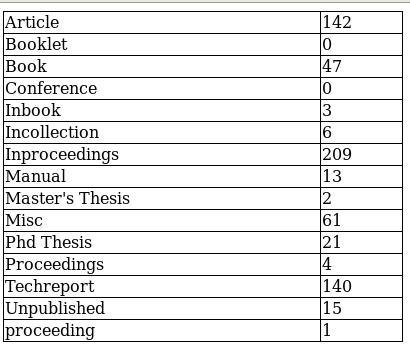
\includegraphics[scale=0.5]{./testes/res_html}
	\caption{Resultado visto no \emph{Firefox}}
	\label{fig:res1}
\end{figure}

A partir do documento que adveio da URL na secção \emph{Resultados}, podemos
constar que não existem entradas que difiram do \hologo{BibTeX}, a não ser
a entrada \emph{proceeding}, e que não existem \emph{Booklets}, nem
\emph{Conferences}. 


\subsection{Alternativas, Decisões e Problemas de Implementação}

Numa primeira implementação, existia uma \emph{trie} para guardar os tipos de
entrada que não pertencessem ao \hologo{BibTeX}. A travessia desta estrutura
é recursiva, embora linear no número de nodos, cada nodo podia ter um
\emph{array} de apontadores de tamanho 256, podendo esse \emph{array} ter poucas
posições ocupadas. De igual modo, a \emph{trie} que estava implementada não
estava otimizada e poderia ter \emph{bugs}. Daí a escolha passar a ser uma
tabela de \emph{hash}. Esta última estrutura, à semelhança da \emph{trie}---
ignorando o tamanho da \emph{string} que compõe a chave ---, continua a ter
tempo constante de inserção, e o \emph{overhead} é menor.

À data de redação deste relatório, chegou-se a conclusão que poder-se-ia ter
escolhido uma tabela de \emph{hash} em \emph{open adressing} ou outra estrutura
otimizada, podendo assim ter um filtro mais eficiente. Futuramente, poder-se-á
tentar utilizar uma estrutura diferente e efetuar mais testes.


